\section{Results} \label{sec:Results}

\begin{figure}
\captionsetup[subfigure]{labelformat=empty}
\captionsetup[subfigure]{justification=centering}
\begin{subfigure}{0.2\textwidth}
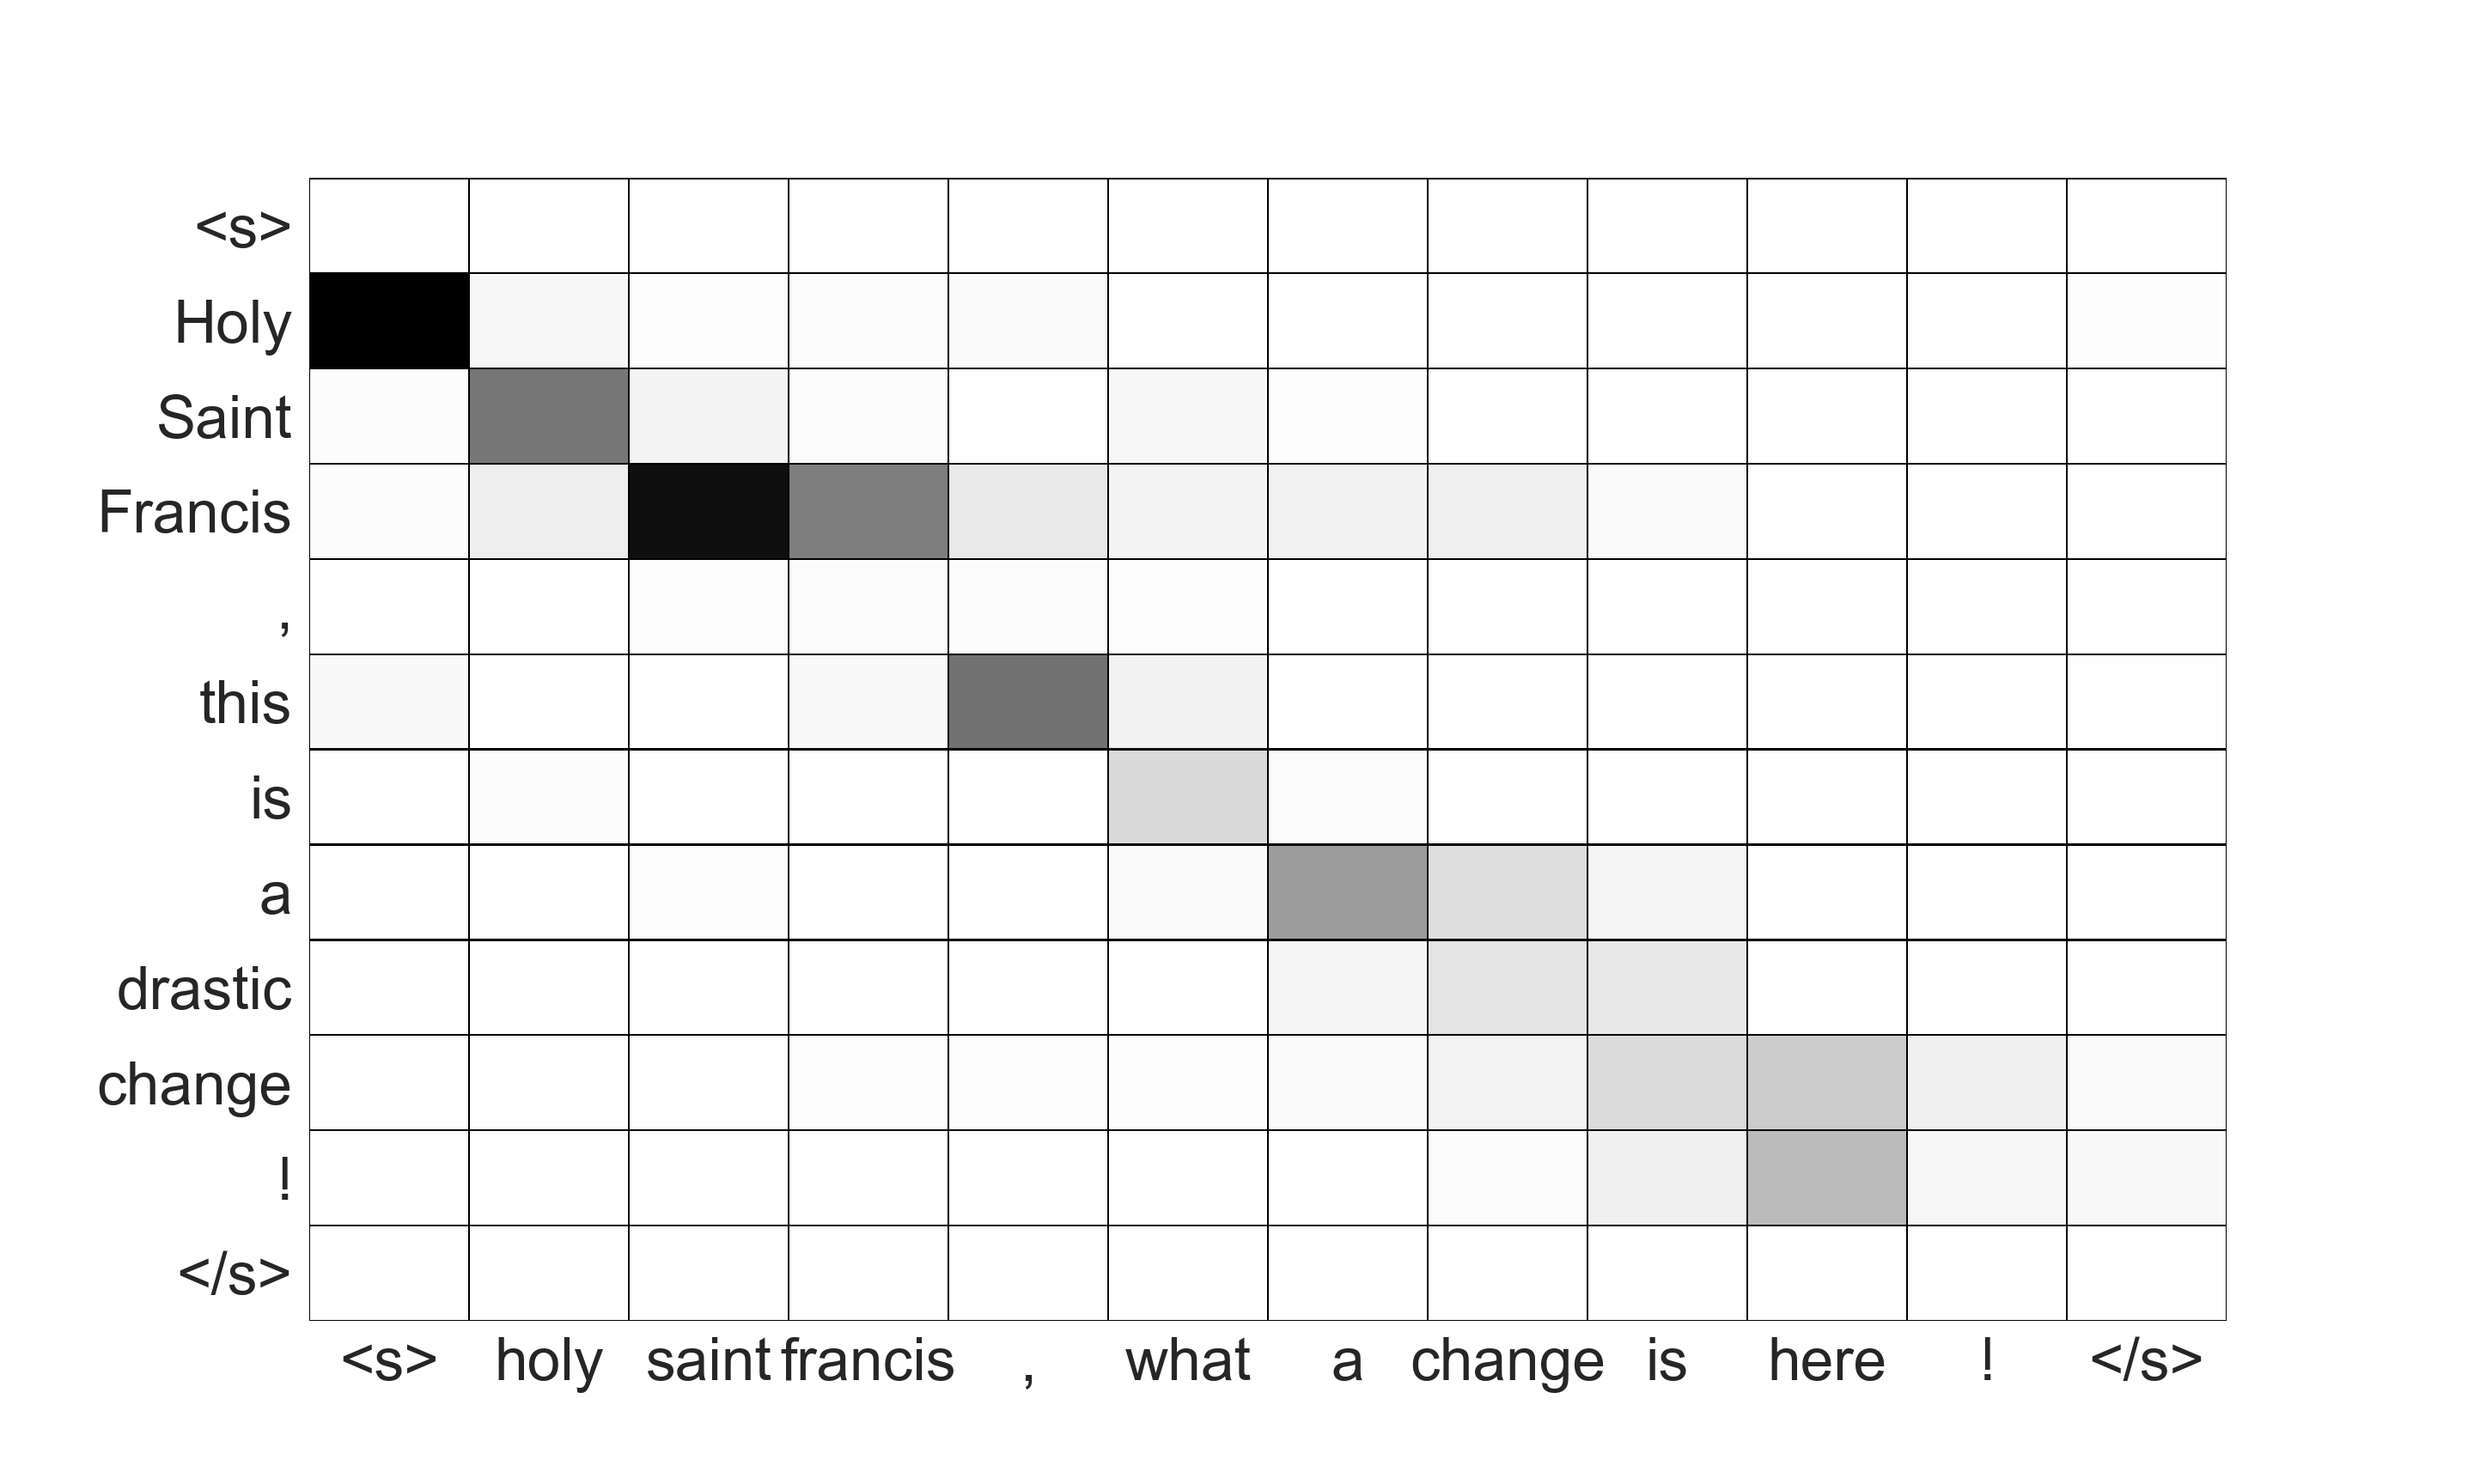
\includegraphics[scale=0.20]{HolySaintFrancisCopy.png}
%\captionsetup{format=hang}
%\caption{Copy Model}
%\label{fig:attention}
\end{subfigure} \hspace{0.15\textwidth}
\begin{subfigure}{0.2\textwidth}
\centering
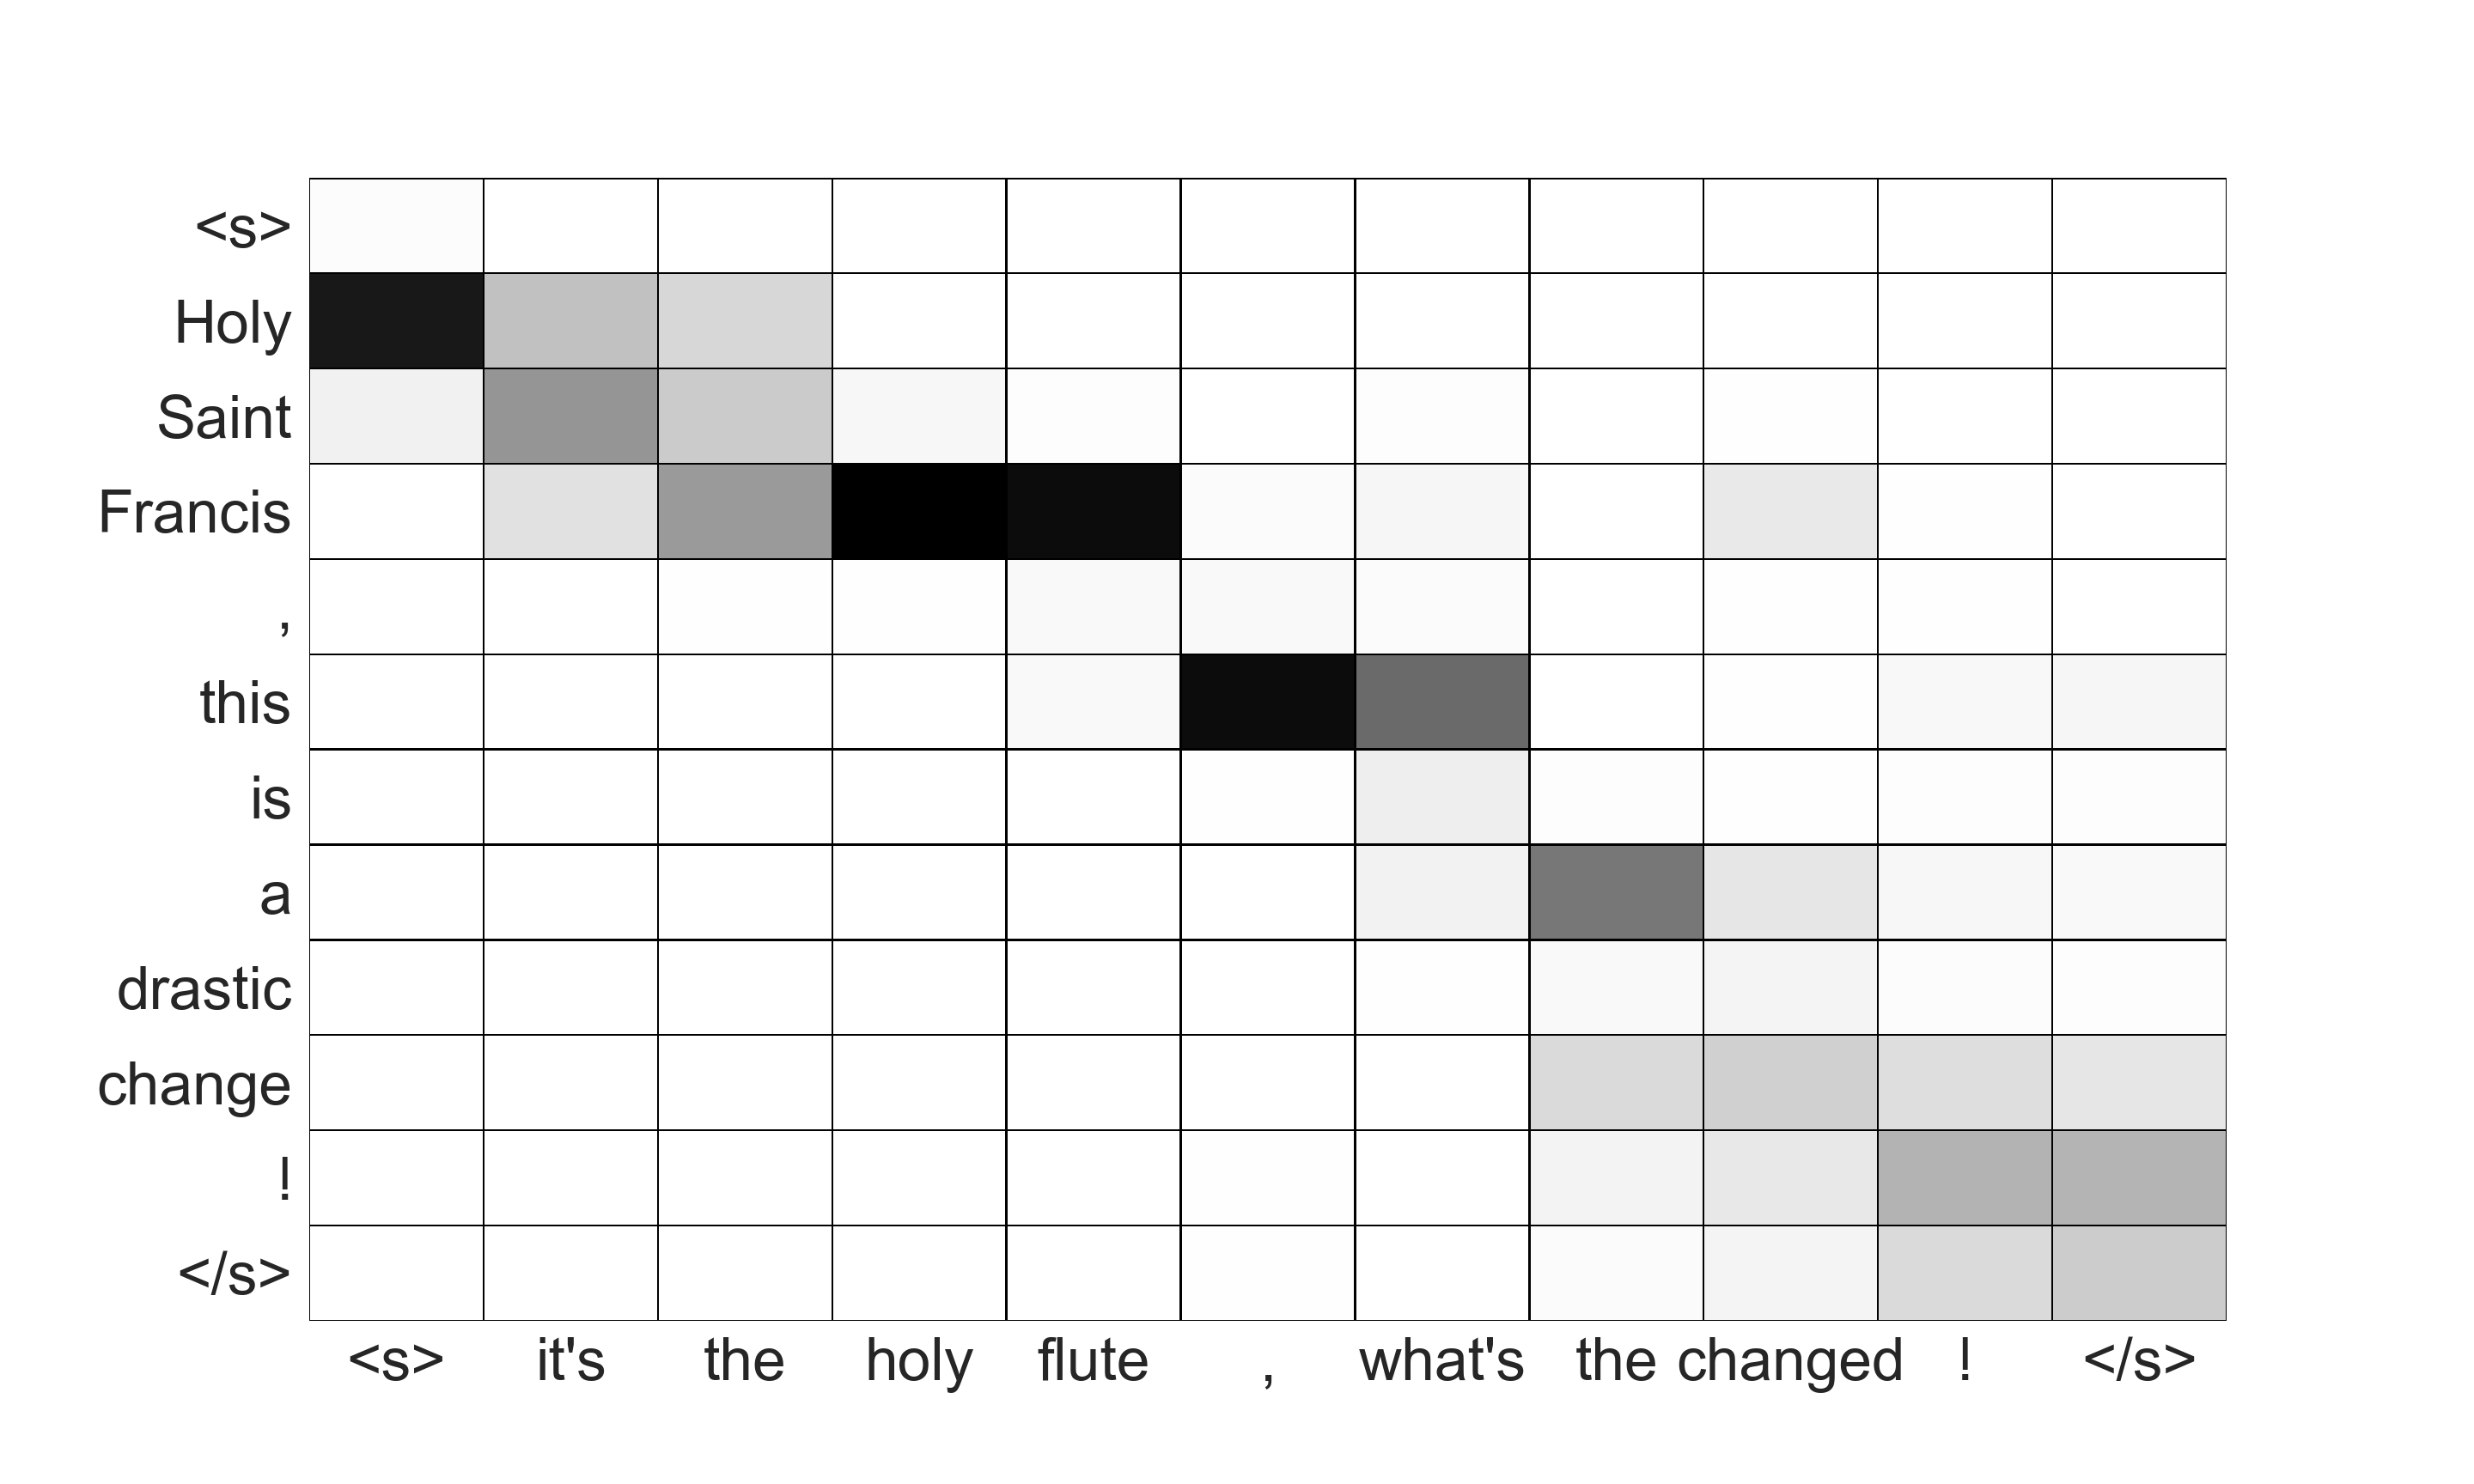
\includegraphics[scale=0.20]{HolySaintFrancisS2S.png}
%\caption{}
%\label{fig:attention2}
\end{subfigure}
\caption{Attention matrices from a \emph{Copy} (top) and a \textit{simple S2S} (bottom) model respectively on the input sentence \textit{``Holy Saint Francis, this is a drastic change!"} . \textbf{$<s>$} and \textbf{$</s>$} are  start and stop characters. Darker cells are higher-valued.}
\textbf{\label{fig:attention}}
\end{figure}

%- BLEU and other measures
%
%- baseline
%- rnn soft attention
%- pointer copy
%- sentinel loss


%Pretrained embeddings
%- different versions
%- trainable vs. non trainable


%Qualitative results
%- good examples, bad examples
%- examples demonstrating copy
The results in Table \ref{tab:knightExp} confirm most of our hypotheses about the right architecture for this task.
\begin{itemize}
    \item \textbf{Copy component}: We can observe from Table \ref{tab:knightExp} that the various \emph{Copy} models each outperform their \emph{SimpleS2S} counterparts by atleast 7-8 BLEU points.
    \item \textbf{Retrofitting dictionary constraints}: The \emph{Retro} configurations generally outperform their corresponding \emph{Plain} configurations. For instance, our best configuration \emph{Copy.Yes.RetroExtFixed} gets a better BLEU than \emph{Copy.Yes.PlainExtFixed} by a margin of atleast 11.
    \item \textbf{Sharing Embeddings}: Sharing source and target side embeddings benefits all the \emph{Retro} configurations, although it slightly deteriorates performance (about 1 BLEU point) for some of the \emph{Plain} configurations. 
    \item \textbf{Fixing Embeddings}: \emph{Fixed} configurations always perform better than corresponding \emph{Var} ones (save some exceptions). For instance, \emph{Copy.Yes.RetroExtFixed} get a BLEU of 31.12 compared to 20.95 for \emph{Copy.Yes.RetroExtVar}. Due to fixing embeddings, the former has just half as many parameters as the latter (5.25M vs 9.40M)
    \item \textbf{Effect of External Data}: Pretraining with external data \emph{Ext} works well along with retrofitting \emph{Retro}. For instance, \emph{Copy.Yes.RetroExtFixed} gets a BLEU improvement of 2+ points over \emph{Copy.Yes.RetroFixed}
    \item \textbf{Effect of Pretraining}: For the \emph{SimpleS2S} models, pre-training adversely affects BLEU. However, for the \emph{Copy} models, pre-training leads to improvement in BLEU. The simplest pretrained \emph{Copy} model, \emph{Copy.No.PlainVar} has a BLEU score 1.8 higher than \emph{Copy.No.NoneVar}.
    \item \textbf{PINC scores}: All the neural models have higher PINC scores than the statistical and dictionary approaches, which indicate that the target sentences produced differ more from the source sentences than those produced by these approaches.
    \item \textbf{Sentinel Loss:} Adding the sentinel loss does not have any significant effect, and ends up reducing BLEU by a point or two, as seen with the \emph{Copy+SL} configurations.
\end{itemize}

\subsection{Qualitative Analysis}
Figure \ref{fig:attention} shows the attention matrices from our best \textit{Copy} model (\emph{Copy.Yes.RetroExtFixed}) and our best \textit{SimpleS2S} model (\emph{SimpleS2S.Yes.Retrofixed}) respectively for the same input test sentence. Without an explicit \textit{Copy} component, the \textit{SimpleS2S} model cannot predict the words \textit{saint} and \textit{francis}, and drifts off after predicting incorrect word \textit{flute}.

Table \ref{tab:intro} presents model outputs\footnote{All neural outputs are lowercase due to our preprocessing. Although this slightly affects BLEU, it helps prevent token occurrences getting split due to capitalization.} for some test examples. In general, the \textit{Copy} model outputs resemble the ground truth more closely compared to \textit{SimpleS2S} and \textit{Stat} . In some cases, it faces issues with repetition (Examples 5 and 7) and fluency (Example 9).
